\documentclass[]{article}

\usepackage{caption}
\usepackage{subcaption}
\usepackage{graphicx}
\usepackage{float}
\usepackage{url}
\usepackage{amsmath}
\usepackage{amssymb}
\usepackage{amsthm}
\usepackage{tocloft}
\usepackage{cancel}
\usepackage{thmtools}
\usepackage{gensymb}
\usepackage{braket}
\usepackage{tikz-feynman}
\usepackage{tikz}
\usepackage{mathtools}
\usepackage{color}
\usepackage{colortbl}
\usepackage[toc,nonumberlist]{glossaries}
\usepackage{glossaries-extra}
\usepackage[T1]{fontenc}
\usepackage[utf8]{inputenc}
\usepackage[toc,page]{appendix}
\newcommand\numberthis{\addtocounter{equation}{1}\tag{\theequation}}
\newcommand{\Lagr}{\mathscr{L}}
\newtheorem{thm}{Theorem}
\newtheorem{defn}[thm]{Definition}
\newtheorem{cor}[thm]{Corollary}
\newtheorem{lemma}[thm]{Lemma}
\graphicspath{{figs/}}
\widowpenalty10000
\clubpenalty10000
\setcounter{tocdepth}{2}

%opening
\title{Theoretical Minimum\\Cosmology}
\author{Simon Crase (compiler)\\simon@greenweaves.nz}

\makeglossaries

\begin{document}

\maketitle

\begin{abstract}
	These are my notes for the \emph{Cosmology}\cite{susskind2013cosmology} lectures from Leonard Susskind's \emph{Theoretical Minimum} series\cite{susskind2007theoretical}. 
	
	Disclaimer: I have created these notes as an aide-m\'emoire for my own use; if you find them useful, you are welcome, but I'd appreciate hearing from you. They are not intended 
	as a substitute for listening to the lectures. The intellectual property for all material derived from the lectures belongs, of course, to Professor Susskind; any mistakes, however, are my own.
	
	The notes were created using TexStudio\cite{TexStudio}, and the bibliography using JabRef\cite{Jabref}.
\end{abstract}

\tableofcontents
\listoffigures
\listoftables
\listoftheorems

\newglossaryentry{gls:isotropic}{
	name={isotropic},
	description={Same in all directions.}}

\newglossaryentry{gls:homogenous}{
	name={homogenous},
	description={Same in every place.}}
		
\section{The expanding (Newtonian) universe}

Cosmology as a science dates back to the discovery of the microwave radiation from the Big Bang in the 1960s. Before that Cosmology was more like natural science--classifying oddities. Thinking of the universe as a physical system, as a system to study mathematically, with a set of physical principles and a set of equations is relatively new.

We will study the universe as a physical system, i.e. something we can study with equations.

\begin{itemize}
	\item First observation: the universe is \gls{gls:isotropic}, averaging over patches of the sky, so it should be \gls{gls:homogenous}. If not we'd have shells centered on Earth!

	\item There are around $10^{11}$ galaxies within view of Earth, which we can treat as particles. Each galaxy has roughly $10^{11}$ stars.
	
	\item Gravity is only force that matters at cosmological scales: it pulls stuff together. Should stuff remain static?
\end{itemize}

Could Newton have figured out expanding universe given observations?

\subsection{How would Newton have handled expanding universe?}

\begin{figure}[H]
	\begin{center}
		\caption{We start by introducing a set of coordinates.}
		\begin{subfigure}[t]{0.45\textwidth}
			\caption{Chose grid so that galaxies are at grid points, so grid moves with galaxies. Galaxies move coherently (from observation).}\label{fig:cosmo-1-grid}
			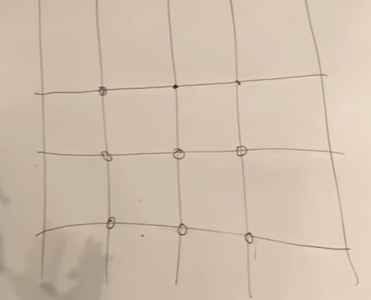
\includegraphics[width=0.8\textwidth]{cosmo-1-grid}
		\end{subfigure}
		\;
		\begin{subfigure}[t]{0.45\textwidth}
			\caption{Define distance: $D_{ab}=a(t) \Delta x_{ab}$, where scale parameter $a$ may or may not be a constant.}\label{fig:cosmo-1-distance}
			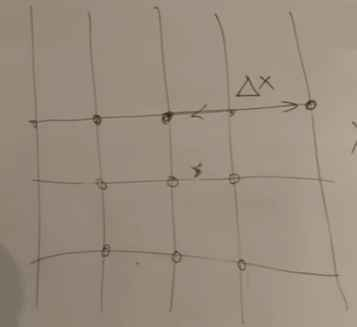
\includegraphics[width=0.8\textwidth]{cosmo-1-distance}
		\end{subfigure}
	\end{center}
\end{figure}
 
 We postulate a more general formula for distance between two galaxies $a$ and $b$:
 
 \begin{align*}            
 	D_{ab}=&a(t) \sqrt{\Delta_{ab} x^2 + \Delta_{ab} y^2 + \Delta_{ab} z^2}  \text{, where $a(t)$ is called the ''scale factor''}
\end{align*}
 Now calculate velocity           
 \begin{align*}	
 	V_{ab}=&\dot{a} \Delta X_{ab} \text{, neglecting $y$ and $z$}\\
 	\frac{V_{ab}}{D_{ab}} =& \frac{\dot{a}}{a} \text{, independent of choice of galaxies!}\\
 	=& H \text{, Hubble constant at a given time.}\\
 	V =& H D \text{, Hubble's Law.}
\end{align*}
 
\subsection{How much mass is in $\Delta x \Delta y \Delta z$?}

Assume  $\Delta x \Delta y \Delta z$ big enough that we can average over the small scale structure. How much mass is in there? Let $M$ denote the mass within $\Delta x \Delta y \Delta z$, and $M = \nu \Delta x \Delta y \Delta z$ Let $V$ denote the volume.

\begin{align*}
	V =& a^3 \Delta x \Delta y \Delta z\\
	M =& \nu \Delta x \Delta y \Delta z \text{, constant}\\
	\rho(t) =& \frac{\nu}{a(t)^3} \numberthis \label{eq:rho}
\end{align*}

Amount of mass in a given region of Figure \ref{fig:cosmo-1-grid} remains the same, as galaxies move with grid.

Chose grid to Newton at rest at centre of universe. He looks out at distant galaxy, which move in accordance with Newton's laws. He would use Newton's Theorem--Figure \ref{fig:newtons:thm}.

\begin{figure}[H]
	\caption[Newton's Theorem]{Newton's Theorem: to determine gravitational force on red body, assuming isotropy, draw sphere and calculate force if mass inside concentrated sphere in centre, and ignore mass outside.}\label{fig:newtons:thm}
	\begin{center}
		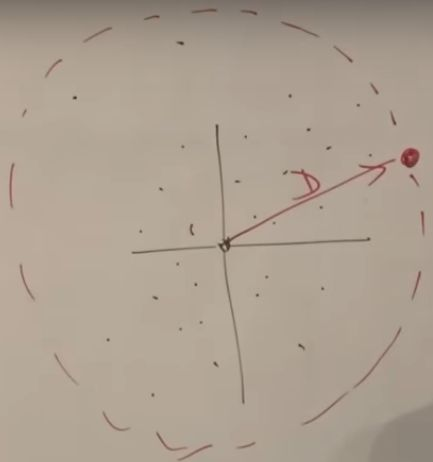
\includegraphics[width=0.8\textwidth]{cosmo-1-newtons-thm}
	\end{center}
\end{figure}

\begin{align*}
	D =& a(t) \sqrt{x^2 + y^2 + z^2}\\
	=&a(t) R \text{, say} \numberthis \label{eq:D}
\end{align*}
R is constant, since galaxy at fixed point in lattice. We want acceleration so we can use Newton's laws.
\begin{align*}
	V =& \dot{a(t)} R\\
	A =& \ddot{a(t)}R
\end{align*}
From Newton's Law of Universal Gravitation
\begin{align*}
	F =& - \frac{mMG}{D^2}\\
	A =& - \frac{MG}{D^2} \text{, which should become}\\
	=& \ddot{a(t)}R
\end{align*}
So we want
\begin{align*}
	\ddot{a(t)}R =& - \frac{MG}{D^2}\\
	=& - \frac{MG}{a^2 R^2} \text{, from \eqref{eq:D}}\\
	\frac{\ddot{a(t)}}{a} =& - \frac{MG}{a^3 R^3}\text{, now volume is}\\
	V =& \frac{4 \pi}{3}  a^3 R^3\\
	\frac{\ddot{a(t)}}{a}=& -\frac{4 \pi}{3} G \rho \text{, from definition of $\rho$} \numberthis \label{eq:a}
\end{align*}

Now $\rho$ does not depend in $R$, so \eqref{eq:a} applies for every galaxy. This is true for any origin, as long as we do the transformation carefully. Everything hinges on the assumption that the universe is homogeneous.

We can see from \eqref{eq:a} that the universe is not static unless $\rho=0$. Let us substitute \eqref{eq:rho} in \eqref{eq:a}.

\begin{align*}
	\frac{\ddot{a(t)}}{a} =& \frac{4 \pi}{3} \frac{G \nu}{a^3}  \numberthis \label{eq:friedmann}
\end{align*}

This was discovered by Friedmann, in the context of General Relativity. It doesn't tell us whether universe is expanding or creating, but tells us that acceleration is negative. But observation says that it isn't! This would have been the standard model before we found that expansion is accelerating.

\begin{figure}[H]
	\caption{Consider throwing rock up from Earth, along x-axis}\label{fig:cosmo:throw:rock}
	\begin{center}
		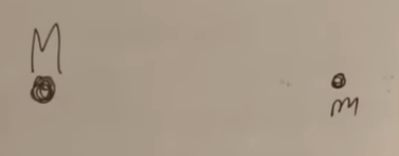
\includegraphics[width=0.5\textwidth]{cosmo-1-throw-rock}
	\end{center}
\end{figure}

We will write down the energy equation: total energy is $\frac{1}{2}m v^2 -\frac{m M G}{x}$. What is escape velocity if total energy is zero?
\begin{align*}
	\frac{1}{2}\cancel{m} V^2 -\frac{\cancel{m} M G}{X} =& 0\\
	V^2 =& \frac{2 M G}{X}
\end{align*}
Similarly in \eqref{eq:friedmann}, total energy can by positive, negative or zero.
\begin{itemize}
	\item If energy great enough, universe does not turn around: it expands forever.
	\item If energy smaller, universe eventually contracts.
	\item Escape velocity is edge.
\end{itemize}

In Figure \ref{fig:newtons:thm}, all the particle knows is that it is moving under influence of mass concentrated at origin, so we can treat as Figure \ref{fig:cosmo:throw:rock}.


\section{Matter and radiation dominated universes}

\section{Geometries of space: flat, spherical, hyperbolic}

\section{Cosmological Thermodynamics}

\section{Vacuum energy}

\section{Dark matter and allocation of energy density}

\section{Temperature History of the Universe}

\section{Baryogenesis}

\section{Inflation}

\section{Inhomogeneities and quantum fluctuations}

% glossary: may need command makeglossaries.exe cosmology
\printglossaries

\bibliographystyle{unsrt}
\addcontentsline{toc}{section}{Bibliography}
\raggedright
\bibliography{tm}

\end{document}
